图\ref{fig:sys.param}给出了Dirty Price与时间t的关系。
\begin{figure}[htbp]
\begin{center}
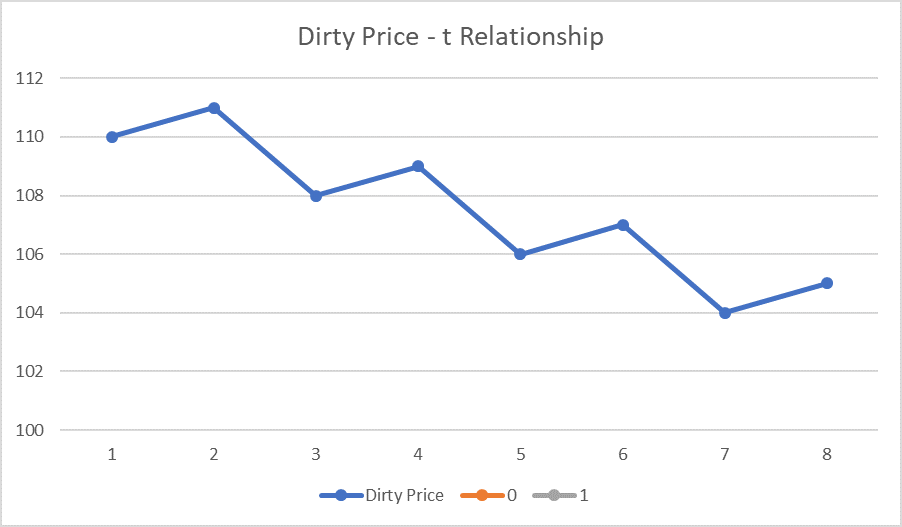
\includegraphics[width=16cm]{img//DirPri_t_Relation.PNG}
\caption{Dirty Price与时间t的关系}
\label{fig:sys.param}
\end{center}
\end{figure}

Dirty price指的是clean price和accrued interest(已经发放的利息)的和。
Clean price指的是还未领取的息票本金折现到当前时刻是多少钱。

其中t坐标轴的偶数(2,4,6,8,……)指的是股息发放日。每次发放股息后,coupon的dirty price等于clean price。随着利息的积累,dirty price逐渐高于clean price,直到下次股息发放日股息再次方法,dirty price再次等于clean price。
市场上的报价通常是clean price,所以交易双方需要根据自己的交易模型计算出accrued interest,在交易时把积累的利息加上去。

对于Duration和convexity,我们有以下结论:
1.Duration的加权平均就是该coupon bond的加权平均
2.Convexity 的加权平均就是该coupon bond的加权平均

规范化表示:
$Duration_avg=(P*V_1*D_1+P*V_2*D_2+ \cdots)/(P*V_1+P*V_2+\cdots)$
$Convexity_avg=(P*V_1*C_1+P*V_2*C_2+\cdots)/(P*V_1+P*V_2+\cdots)$

